\section*{\large{Архитектура сервиса}}
\addcontentsline{toc}{section}{Архитектура сервиса}

Для решения задачи генерации векторных тайлов
для набора геоданных предлагается следующая архитектура.

\begin{figure}[H]
	\hspace*{-1 cm}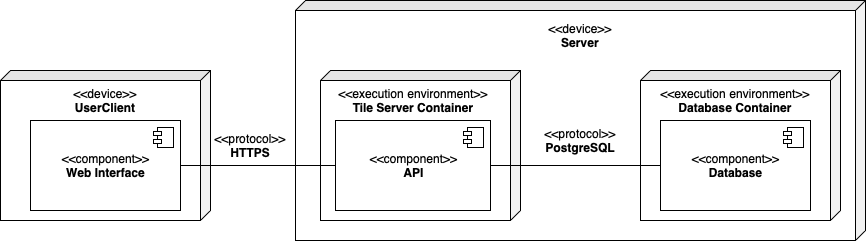
\includegraphics[width=\textwidth, left]{images/architecture/1}
	\caption{Диаграмма размещения}
	\label{pic:architecture__deployment-diagram}
\end{figure}
\vskip 5 mm

\noindent Компоненты представленные на диаграмме размещения (см. рис\ \ref{pic:architecture__deployment-diagram}):
\begin{itemize}
	\item \textbf{Web Interface} -- веб-интерфейс, позволяющий осуществлять взаимодействие с системой пользователю.
	\item \textbf{Tile Server Container}
	\begin{itemize}
		\item API -- веб-сервер, предоставляющий API для получения векторных тайлов.
	\end{itemize}
	\item \textbf{Database Container}
	\begin{itemize}
		\item Database -- база данных (БД), используемая для хранения данных генеральных планов.
	\end{itemize}
\end{itemize}

\begin{figure}[H]
	\hspace*{-2.5 cm}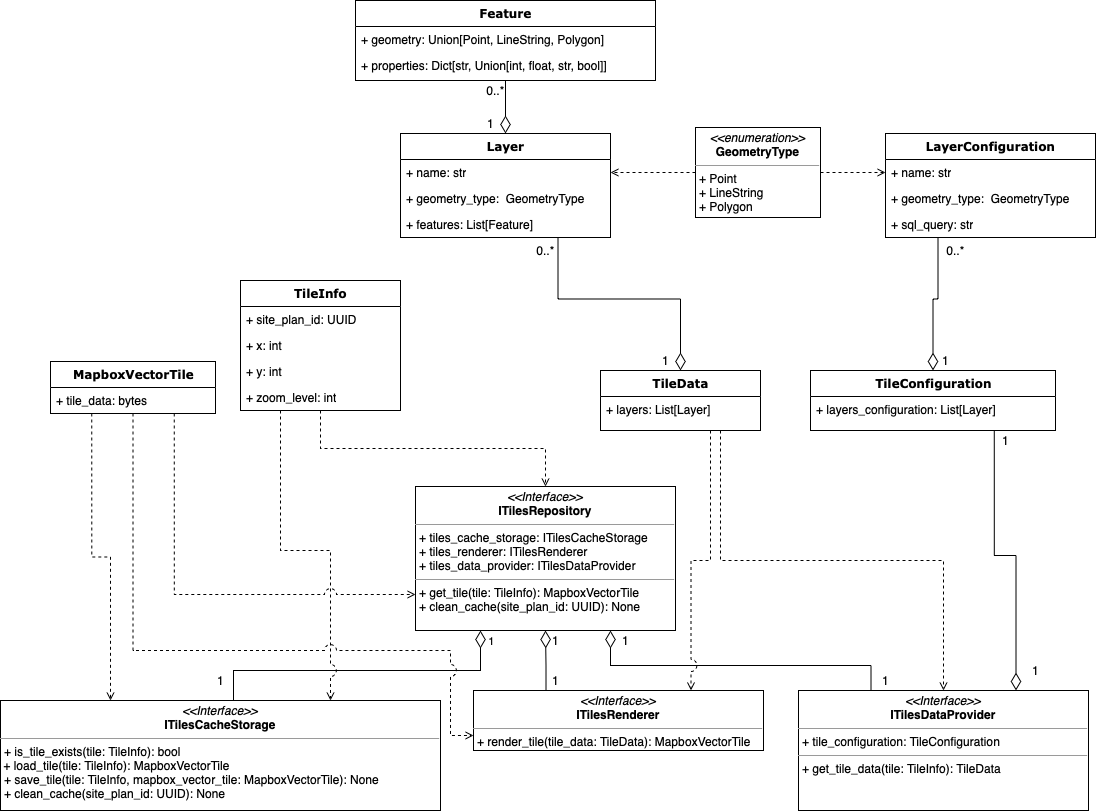
\includegraphics[width=1.2\textwidth, left]{images/architecture/2}
	\caption{Диаграмма классов}
	\label{pic:architecture__classes-diagram}
\end{figure}
\vskip 5 mm
Основное ядро бизнес-логики проекта представлено на диаграмме классов(см. рис\ \ref{pic:architecture__classes-diagram}).
Основные классы и интерфейсы:
\begin{enumerate}
	\item \textit{ITilesCacheStorage} -- сервис, отвечающий за кэширование векторных тайлов.
	\item \textit{ITilesRenderer} -- сервис, отвечающий за рендеринг векторных тайлов.
	\item \textit{ITilesDataProvider} -- сервис, отвечающий за получение данных из внешних источников для рендеринга.
	\item \textit{ITilesRepository} -- оркестратор, отвечает за получение отрендеренных тайлов.
	Если тайла нет в кэше, то он с помощью \textit{ITilesDataProvider} получает данные для рендеринга, потом
	с помощью \textit{ITilesRenderer} рендерит тайлы, а после сохраняет их в кэш \textit{ITilesCacheStorage}.
	\item \textbf{TileInfo} -- хранит в себе координаты запрашиваемого тайла, а также уникальный идентификатор генплана.
	\item \textbf{TileData} -- хранит в себе сырые данные, запрошенные по \textbf{TileInfo}.
	Из сырых данных генерируется \textbf{MapboxVectorTile}.
	\item \textbf{TileConfiguration} -- хранит в себе параметры слоев, которые требуется получить из источника данных.
	\item \textbf{MapboxVectorTile} -- хранит в себе данные, соответствующие спецификации \textit{Mapbox Vector Tile 2.1}.
\end{enumerate}
